%%%%%%%%%%%%%%%%%%%%%%%%%%%%%%%%%%%%%%%%%%%%%%%%%%%%%%%%%
%%%%%%%%%%%%%%%%%%%%%%%%%%%%%%%%%%%%%%%%%%%%%%%%%%%%%%%%%
\section{Qualitative Diagnosis and Prognosis}
\begin{frame}
    \begin{block}{}
        An Application to Prostate Cancer Diagnosis and Prognosis
    \end{block}
\end{frame}
%%%%%%%%%%%%%%%%%%%%%%%%%%%%%%%%%%%%%%%%%%%%%%%%%%%%%%%%%
%%%%%%%%%%%%%%%%%%%%%%%%%%%%%%%%%%%%%%%%%%%%%%%%%%%%%%%%%



%%%%%%%%%%%%%%%%%%%%%%%%%%%%%%%%%%%%%%%%%%%%%%%%%%%%%%%%%
\begin{frame}
\frametitle{Prostate Cancer}
\framesubtitle{The Question is \emph{Will He Outlive It?}}


    \begin{block}{}
        \begin{itemize}
            \item More than $225,000$ cases per year (USA).
            \item One is seven men will be diagnosed.
            \item Treatments: surgery, chemo, radiation, harmone therapy.
            \item Either slowly-growing  and benign or fast-growing
                and dangerous.
            \item Surgery / radiation benefits questionable for SG/B.
            \item Surgery / radiation side effects not desirable.
            \item ... therefore, active surveillance.
        \end{itemize}
    \end{block}

\end{frame}
%%%%%%%%%%%%%%%%%%%%%%%%%%%%%%%%%%%%%%%%%%%%%%%%%%%%%%%%%

%%%%%%%%%%%%%%%%%%%%%%%%%%%%%%%%%%%%%%%%%%%%%%%%%%%%%%%%%
\begin{frame}
\frametitle{Prostate Cancer}
\framesubtitle{Diagnosis}

\centering
    \only<1>{
\includegraphics[width=\textwidth]{gleason/gleason-process-1}}%
    \only<2>{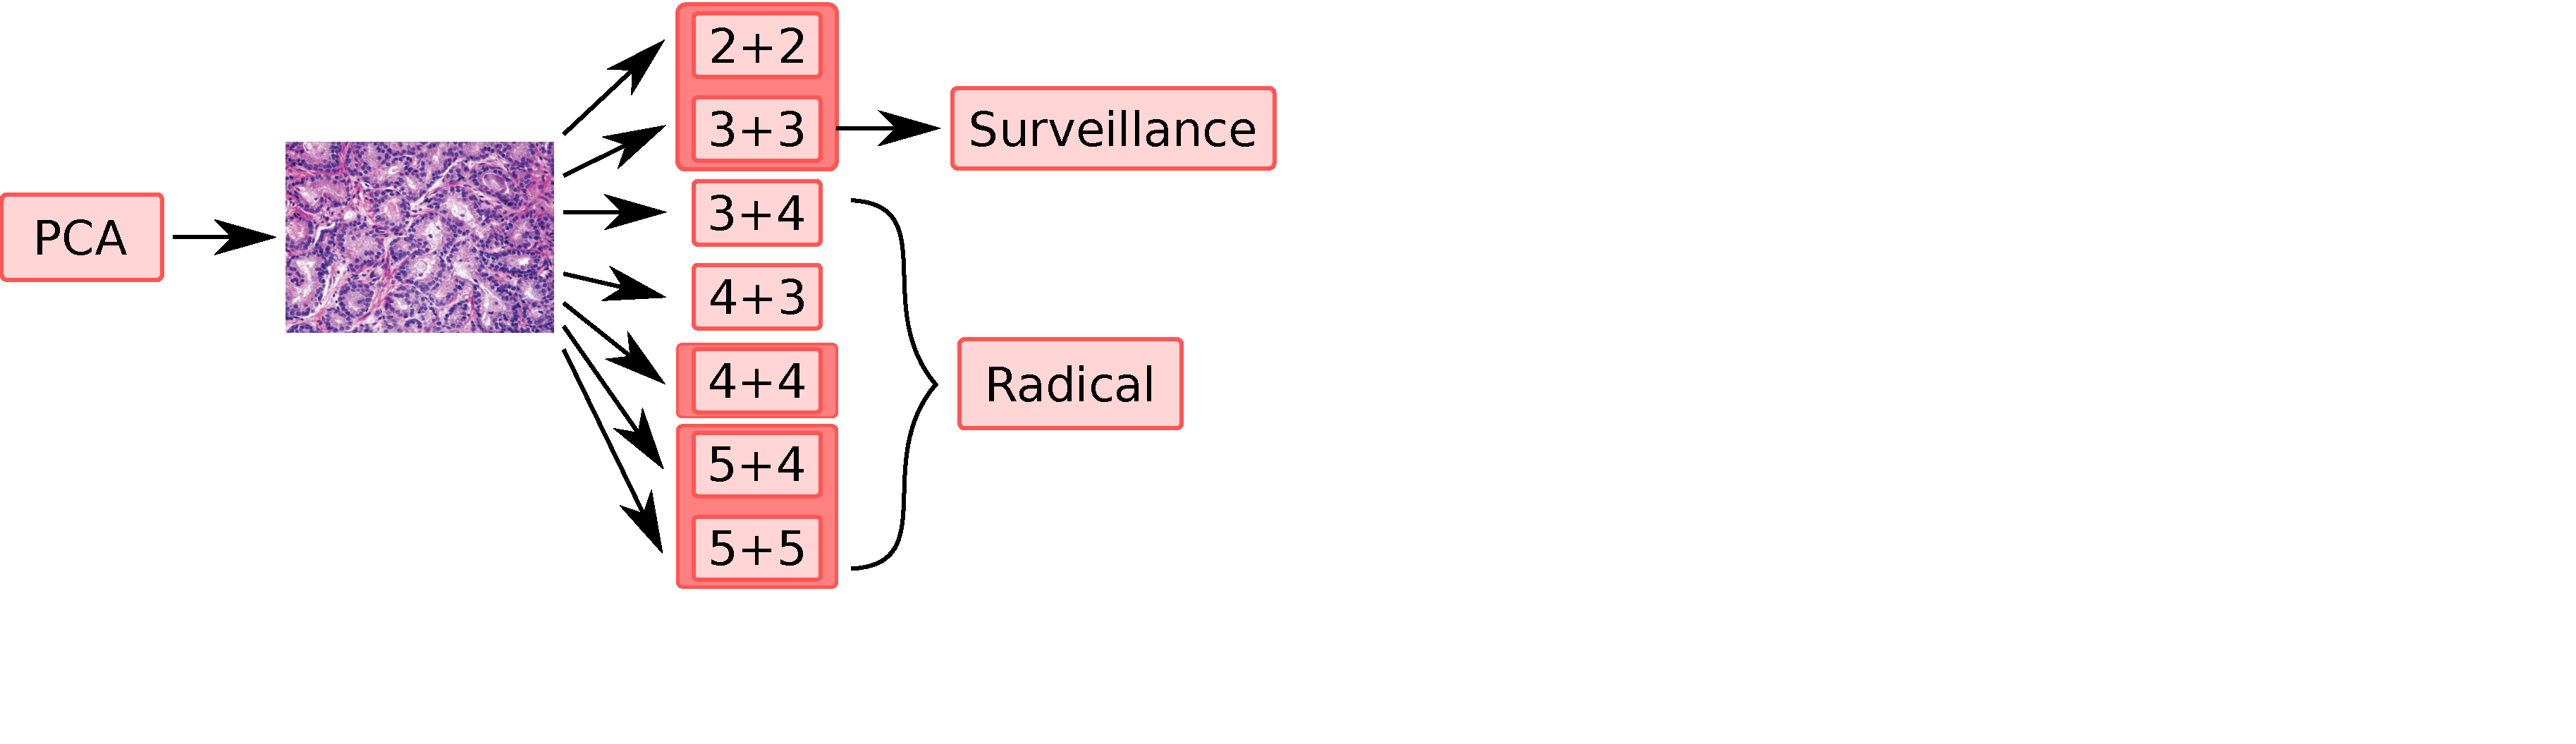
\includegraphics[width=\textwidth]{gleason/gleason-process-2}}%
    \only<3>{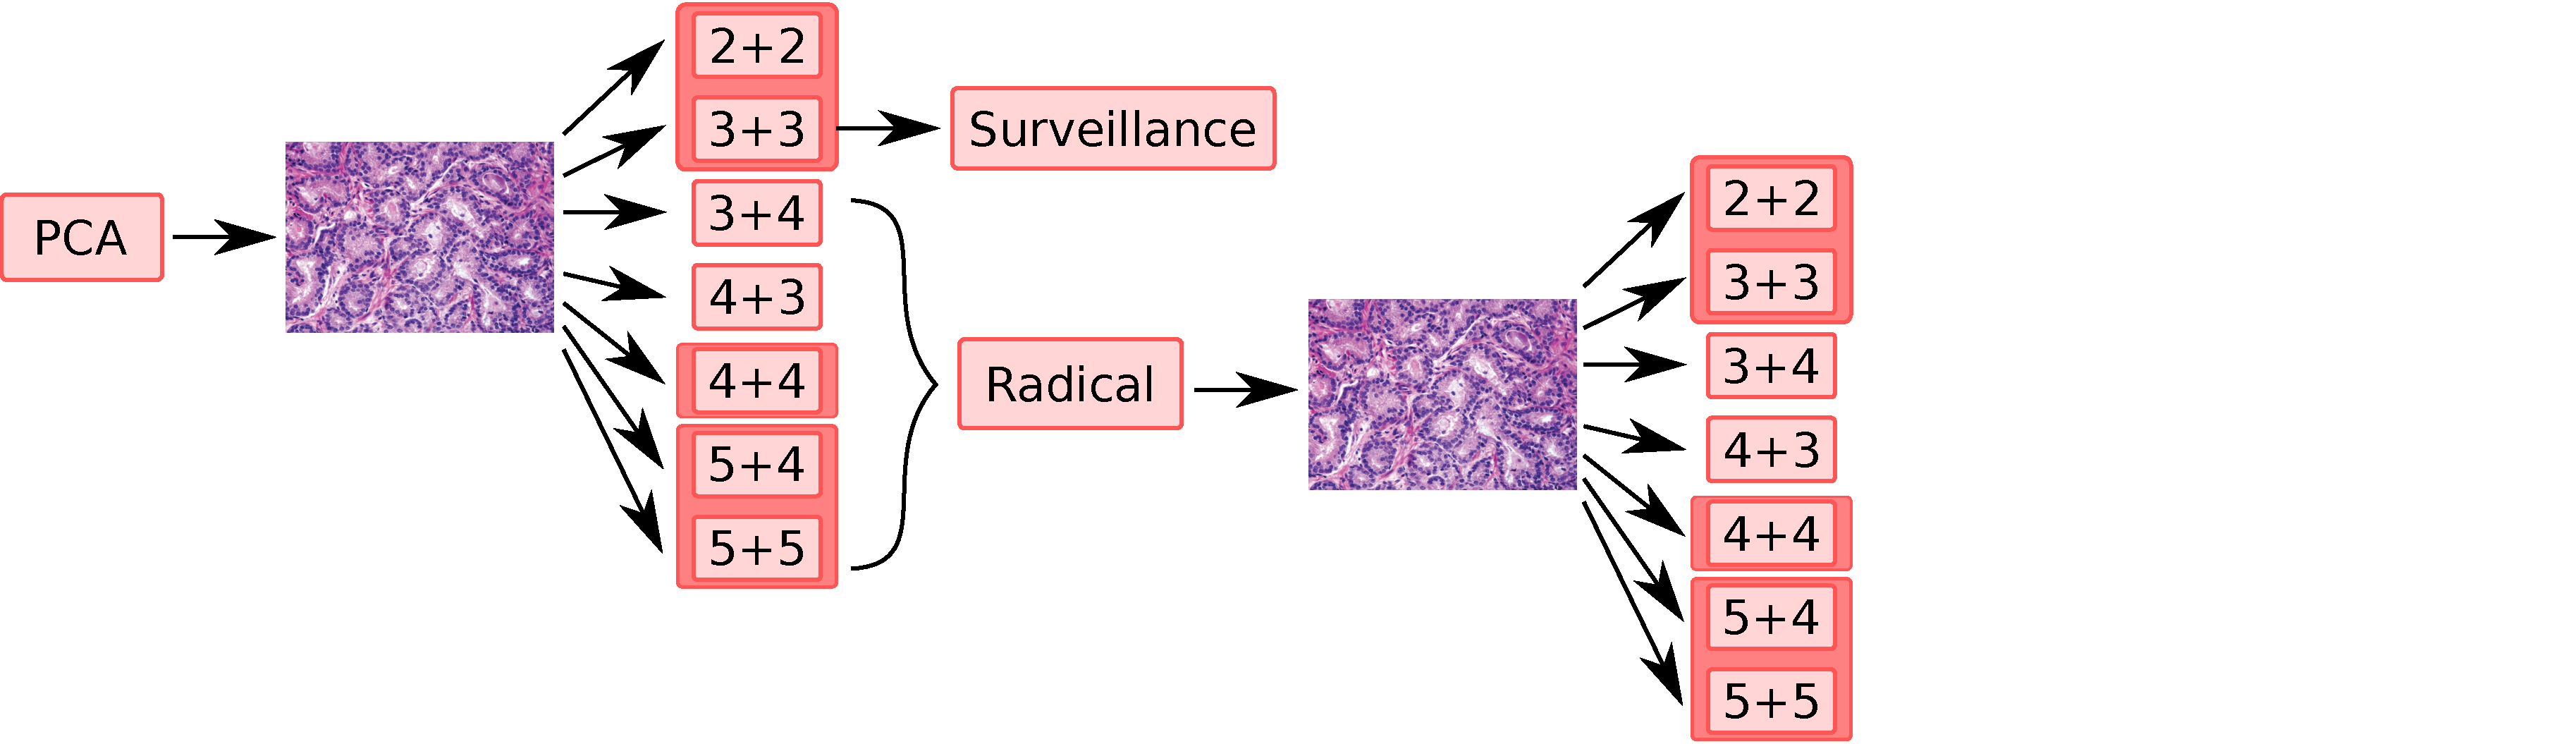
\includegraphics[width=\textwidth]{gleason/gleason-process-3}}%
    \only<4->{\includegraphics[width=\textwidth]{gleason/gleason-process}}

\end{frame}
%%%%%%%%%%%%%%%%%%%%%%%%%%%%%%%%%%%%%%%%%%%%%%%%%%%%%%%%%


%%%%%%%%%%%%%%%%%%%%%%%%%%%%%%%%%%%%%%%%%%%%%%%%%%%%%%%%%
\begin{frame}
\frametitle{Biopsy and Prostectmy Slides}
\framesubtitle{How to Describe Glandular Architecture}

        \centering
        \only<1->{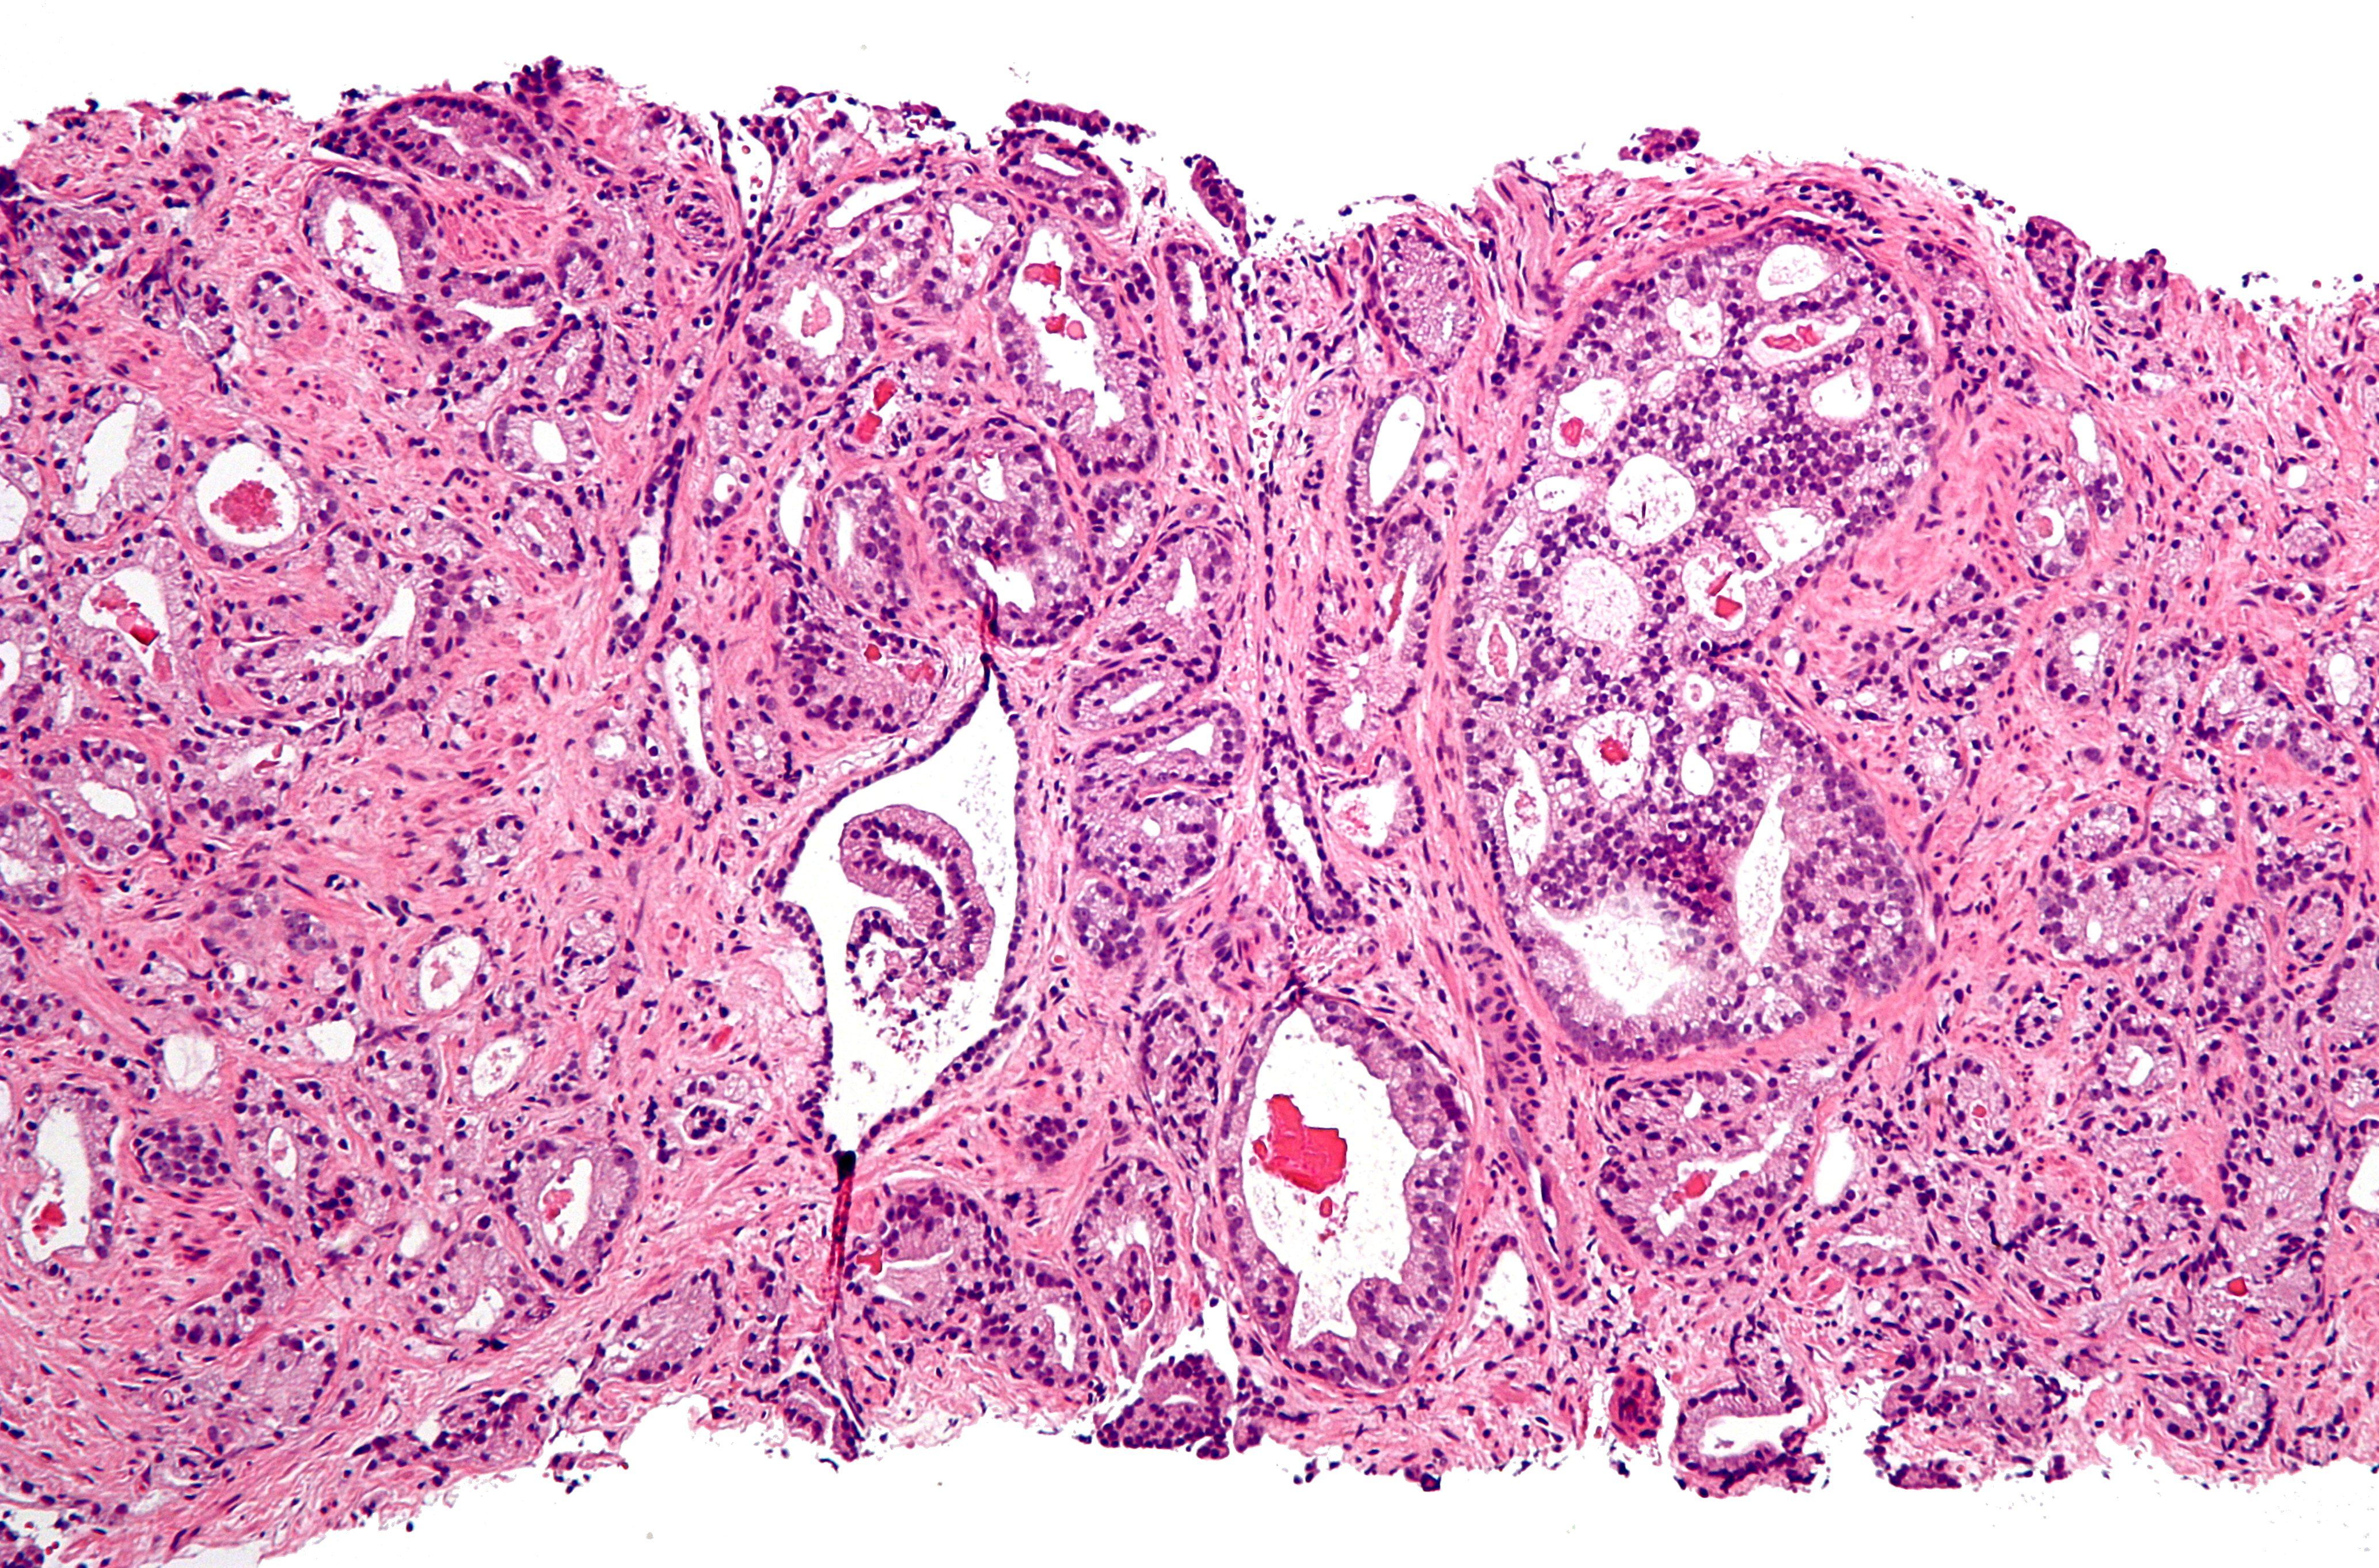
\includegraphics[height=2.5in]{gleason/gleason-4}}

\end{frame}
%%%%%%%%%%%%%%%%%%%%%%%%%%%%%%%%%%%%%%%%%%%%%%%%%%%%%%%%%


%%%%%%%%%%%%%%%%%%%%%%%%%%%%%%%%%%%%%%%%%%%%%%%%%%%%%%%%%
\begin{frame}
\frametitle{Gleason Grading}
\framesubtitle{~}

    \begin{columns}
        \column{.45\textwidth}
        \centering
        \only<1>{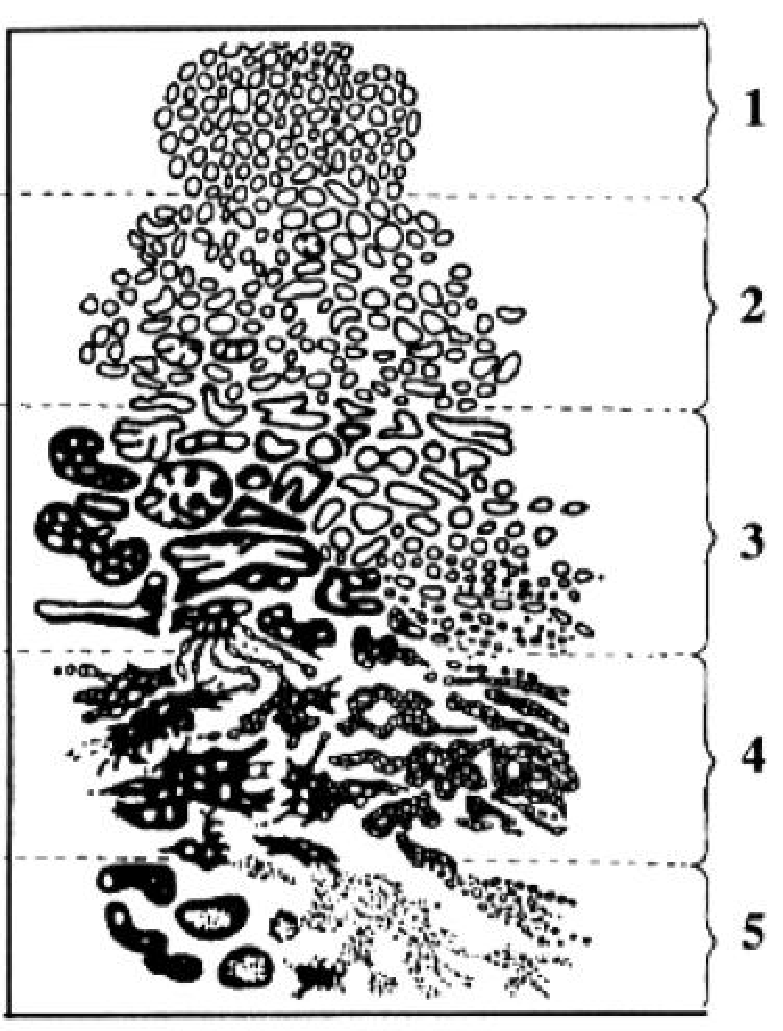
\includegraphics[height=2in]{gleason/gleason}}
        \only<2->{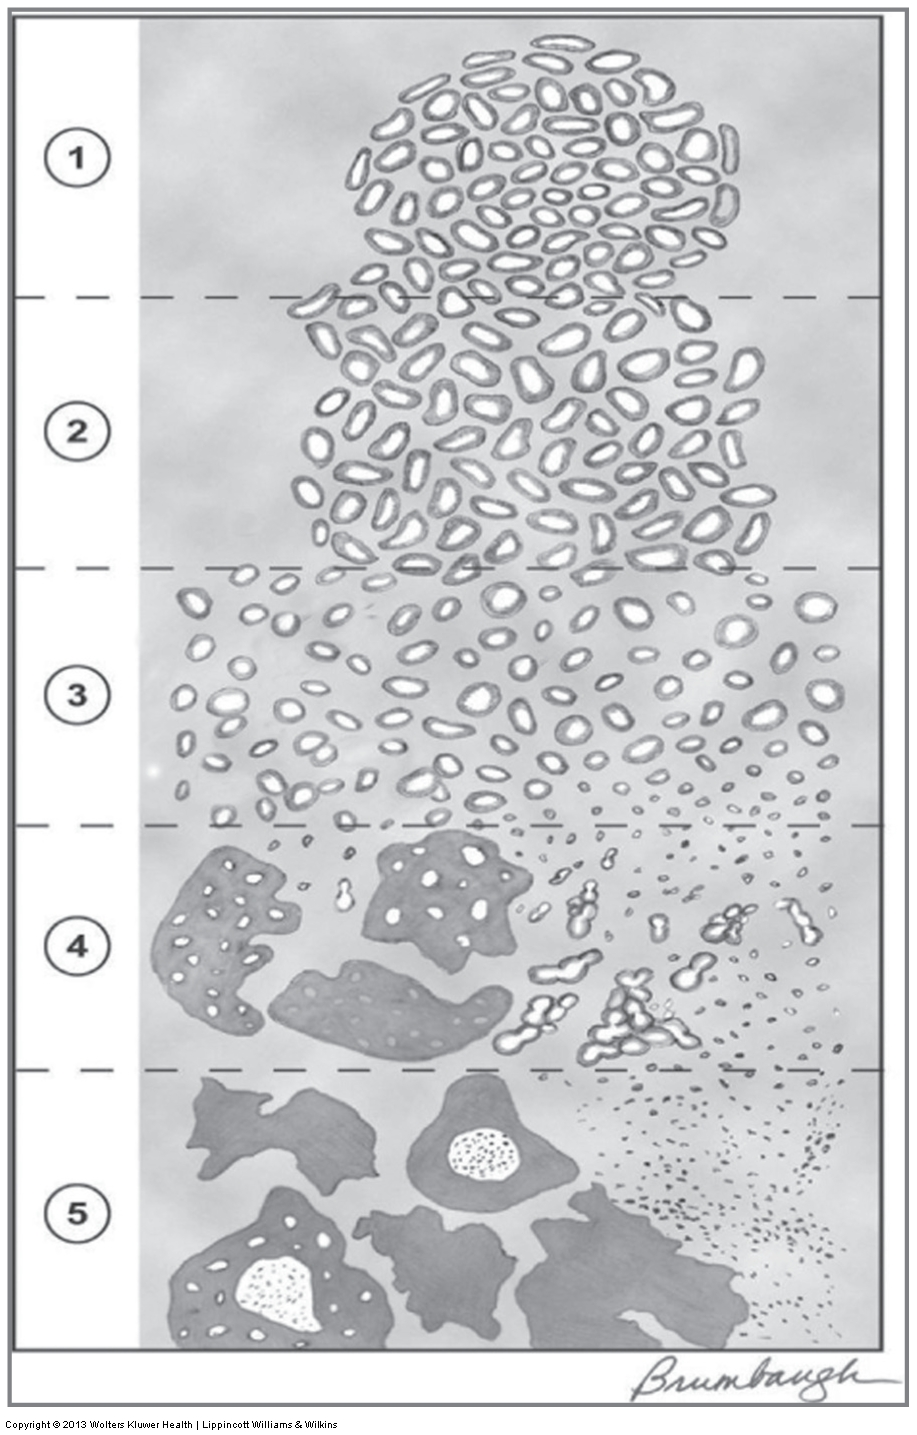
\includegraphics[height=2in]{gleason/epp-figure_1-4}}
        \column{.45\textwidth}
        \begin{block}{}
            \hangindent=1.5cm
            \hangafter=1
            \noindent
            Grade 1: well-defined, nicely packed

            \hangindent=1.5cm
            \hangafter=1
            \noindent
            Grade 2: larger, more tissue,  less uniform

            \hangindent=1.5cm
            \hangafter=1
            \noindent
            Grade 3: less defined glands%
            \only<1>{, some cribriform}

            \hangindent=1.5cm
            \hangafter=1
            \noindent
            Grade 4: fused glands, open lumens%
            \only<2->{, cribriform}

            \hangindent=1.5cm
            \hangafter=1
            \noindent
            Grade 5: no glandular definition, sheets of cells
        \end{block}
    \end{columns}
    \only<1>{\footnotetext{
        Donald Gleason, 1966, image from \emph{The Gleason Grading System: A Complete
        Guide for Pathologist and Clinicians} by Eppstein}}
    \only<2>{\footnotetext{
        2005 Consensus, image from \emph{The Gleason Grading System: A Complete
        Guide for Pathologist and Clinicians} by Eppstein}}

\end{frame}
%%%%%%%%%%%%%%%%%%%%%%%%%%%%%%%%%%%%%%%%%%%%%%%%%%%%%%%%%

\frame{
\frametitle{Recent Updates to Gleason Grading}
\framesubtitle{ISUP 2014}
\begin{block}{'Bears Little Resemblance to the Original Gleason System'}
\begin{itemize}
 \item Rules set for particular glandular features.\pause
 \item Grade group 1: Scores 1-6.
 \item Grade group 2: Score 3+4.
 \item Grade group 3: Score 4+3.
 \item Grade group 4: Scores 8.
 \item Grade group 5: Scores 9-10.\pause
 \item What about tertiary patterns?
 \item ... quantifying the amount of each pattern present?
 \item ... reproducibility?
\end{itemize}

\end{block}
}

%%%%%%%%%%%%%%%%%%%%%%%%%%%%%%%%%%%%%%%%%%%%%%%%%%%%%%%%%
\begin{frame}
    \frametitle{Learning to Grade}
    \framesubtitle{\emph{The Gleason Grading System: A Complete Guide for
    Pathologists and Clinicians}}

    \centering
    
\includegraphics[height=3in]{gleason/gleason-book}

\end{frame}
%%%%%%%%%%%%%%%%%%%%%%%%%%%%%%%%%%%%%%%%%%%%%%%%%%%%%%%%%

%%%%%%%%%%%%%%%%%%%%%%%%%%%%%%%%%%%%%%%%%%%%%%%%%%%%%%%%%
\begin{frame}
\frametitle{Glandular Architecture}
    \framesubtitle{Distribution of Glandular Shape and Size}

    \begin{columns}
        \column{.45\textwidth}
        \centering
        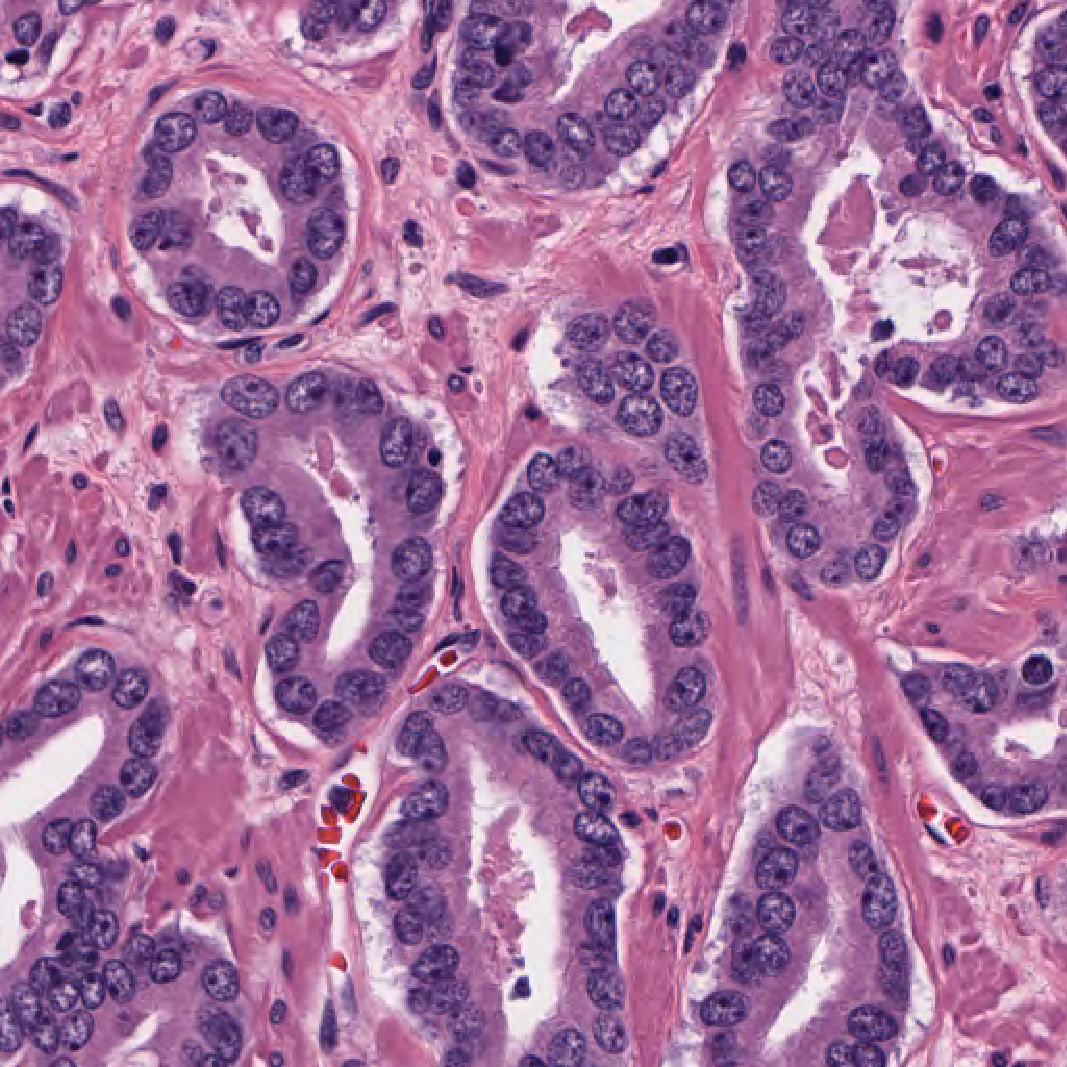
\includegraphics[height=1in]{gleason/gleason3}\\
        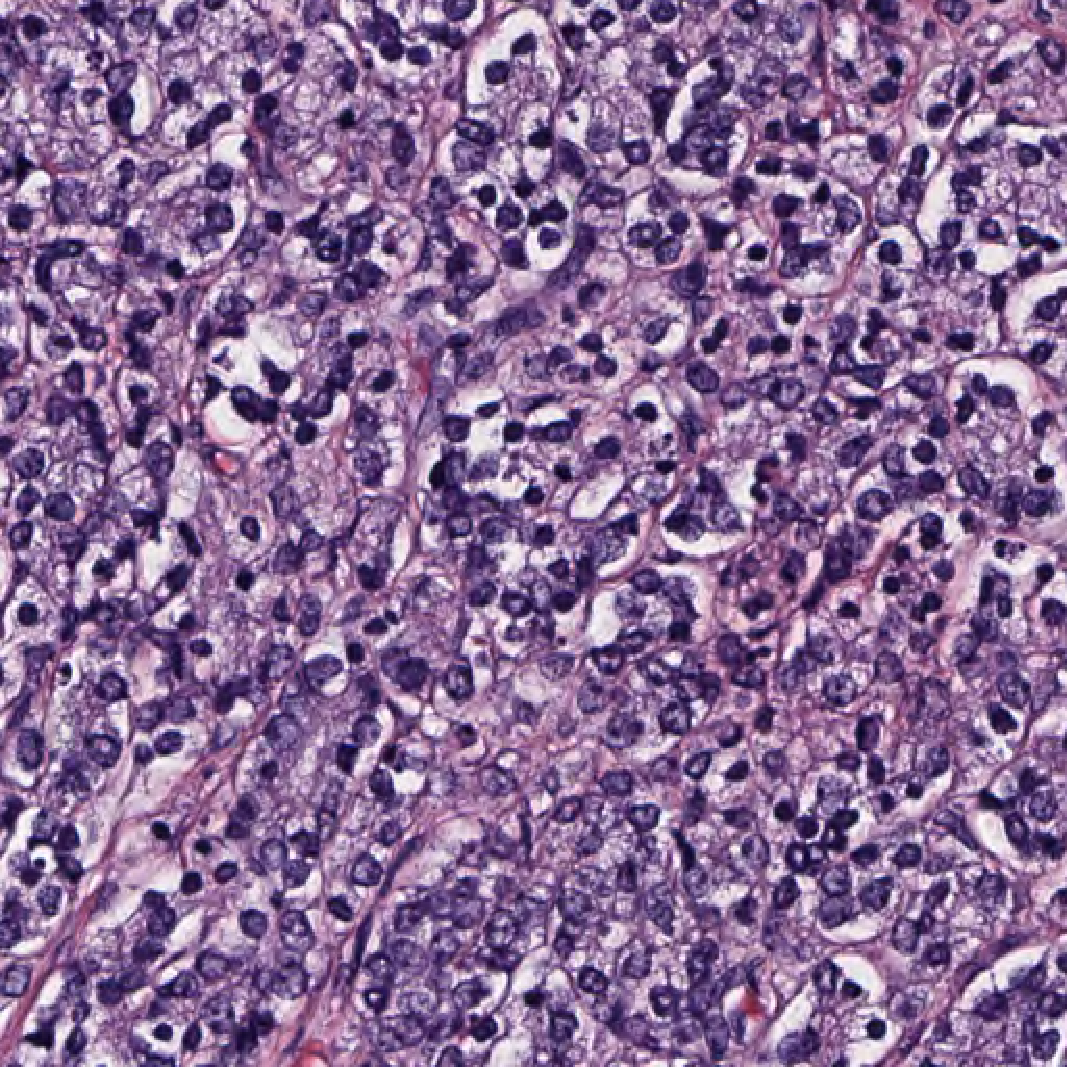
\includegraphics[height=1in]{gleason/gleason5}
        \column{.45\textwidth}
        \begin{block}{Gleason 1}
            Uniform distribution of gland size. Round.
        \end{block}
        \begin{block}{Gleason 3}
            Irregularly separated glands.
        \end{block}
        \begin{block}{Gleason 4}
            Poorly formed glands.
        \end{block}
    \end{columns}
    \only<1->{\footnotetext{Image source: Eppstein, \emph{The Gleason Grading
    System}}}
\end{frame}
%%%%%%%%%%%%%%%%%%%%%%%%%%%%%%%%%%%%%%%%%%%%%%%%%%%%%%%%%

%%%%%%%%%%%%%%%%%%%%%%%%%%%%%%%%%%%%%%%%%%%%%%%%%%%%%%%%%
\subsection{Results}
%%%%%%%%%%%%%%%%%%%%%%%%%%%%%%%%%%%%%%%%%%%%%%%%%%%%%%%%%


\begin{frame}<1>[label=simulated]
    \frametitle{Simulated Data}
    \framesubtitle{Wok with E.\ Berry, Y.C.\ Chen,  J.\ Cisewski-Kehe, S.\ Payne, A.\
    Schenfisch, J.~Schoupbach , N.\ Stouffer.}

    \begin{block}{}
        \centering
        \only<1>{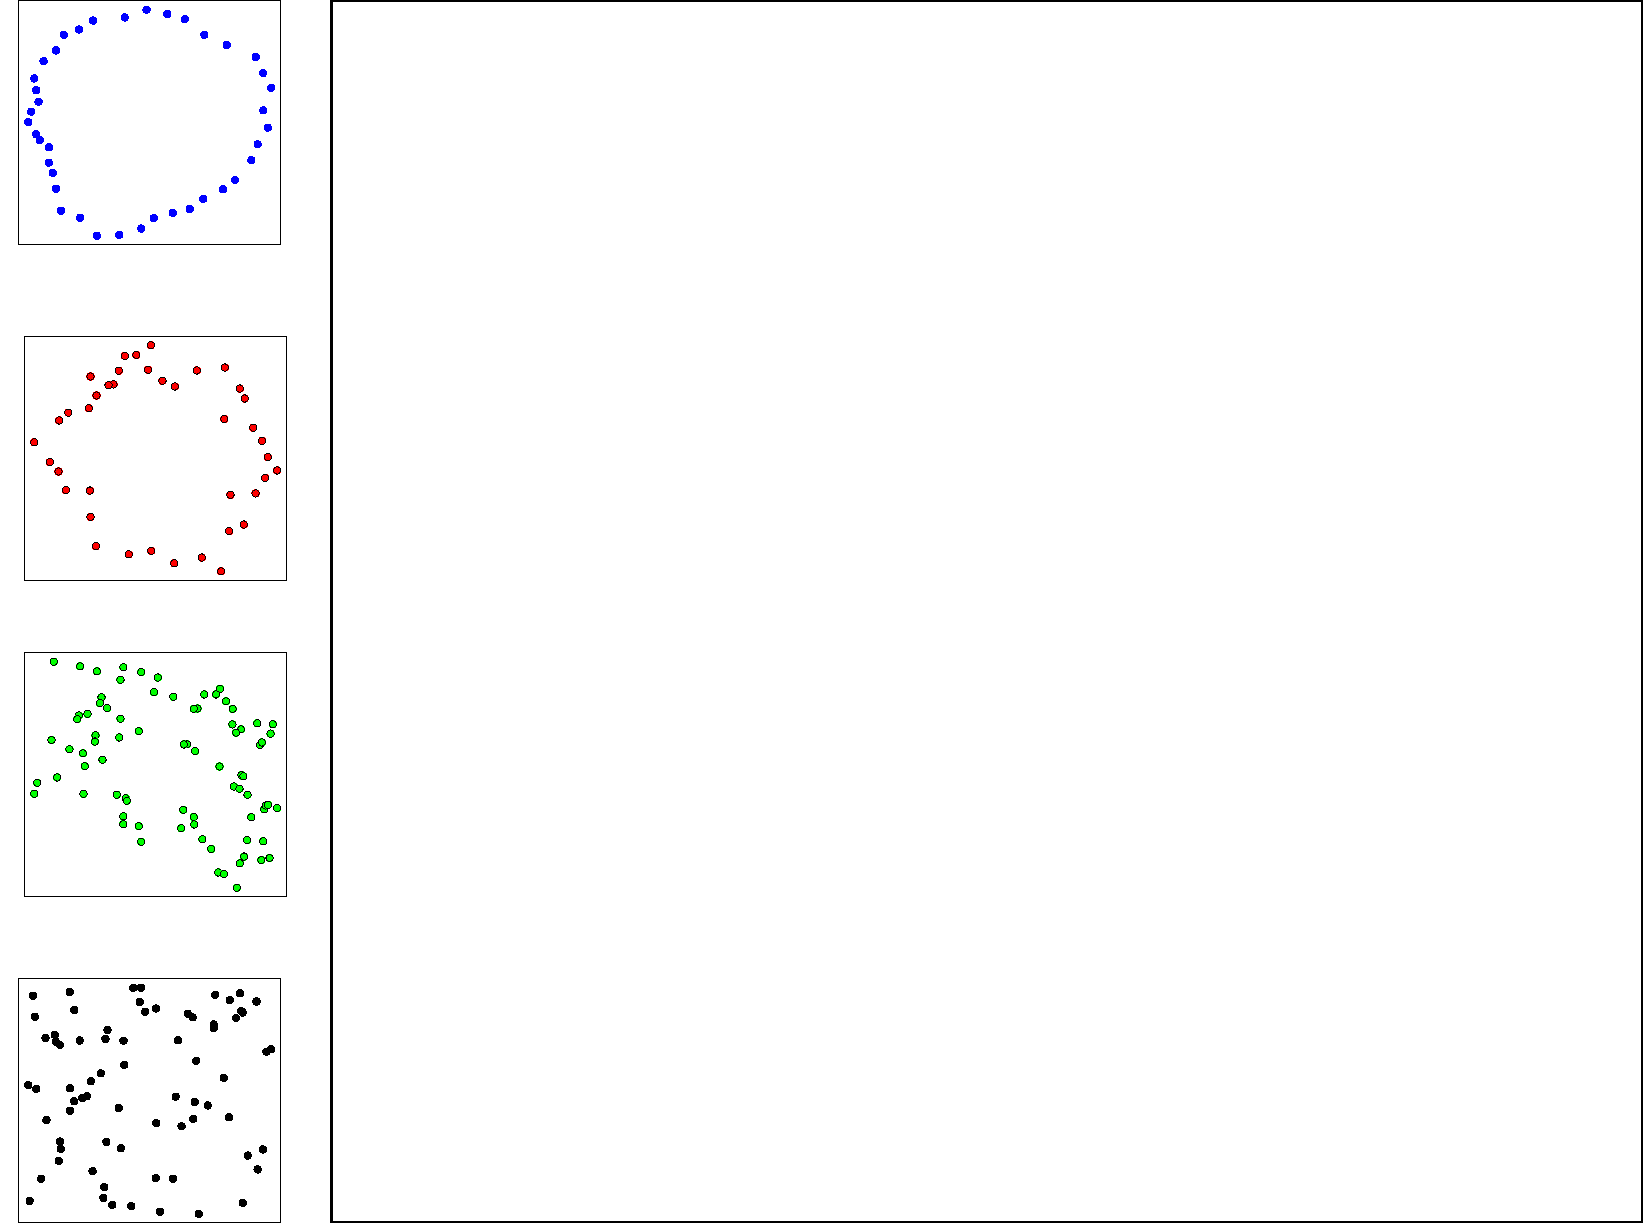
\includegraphics[height=2.5in]{gleason/sil-mds-input}}%
        \only<2->{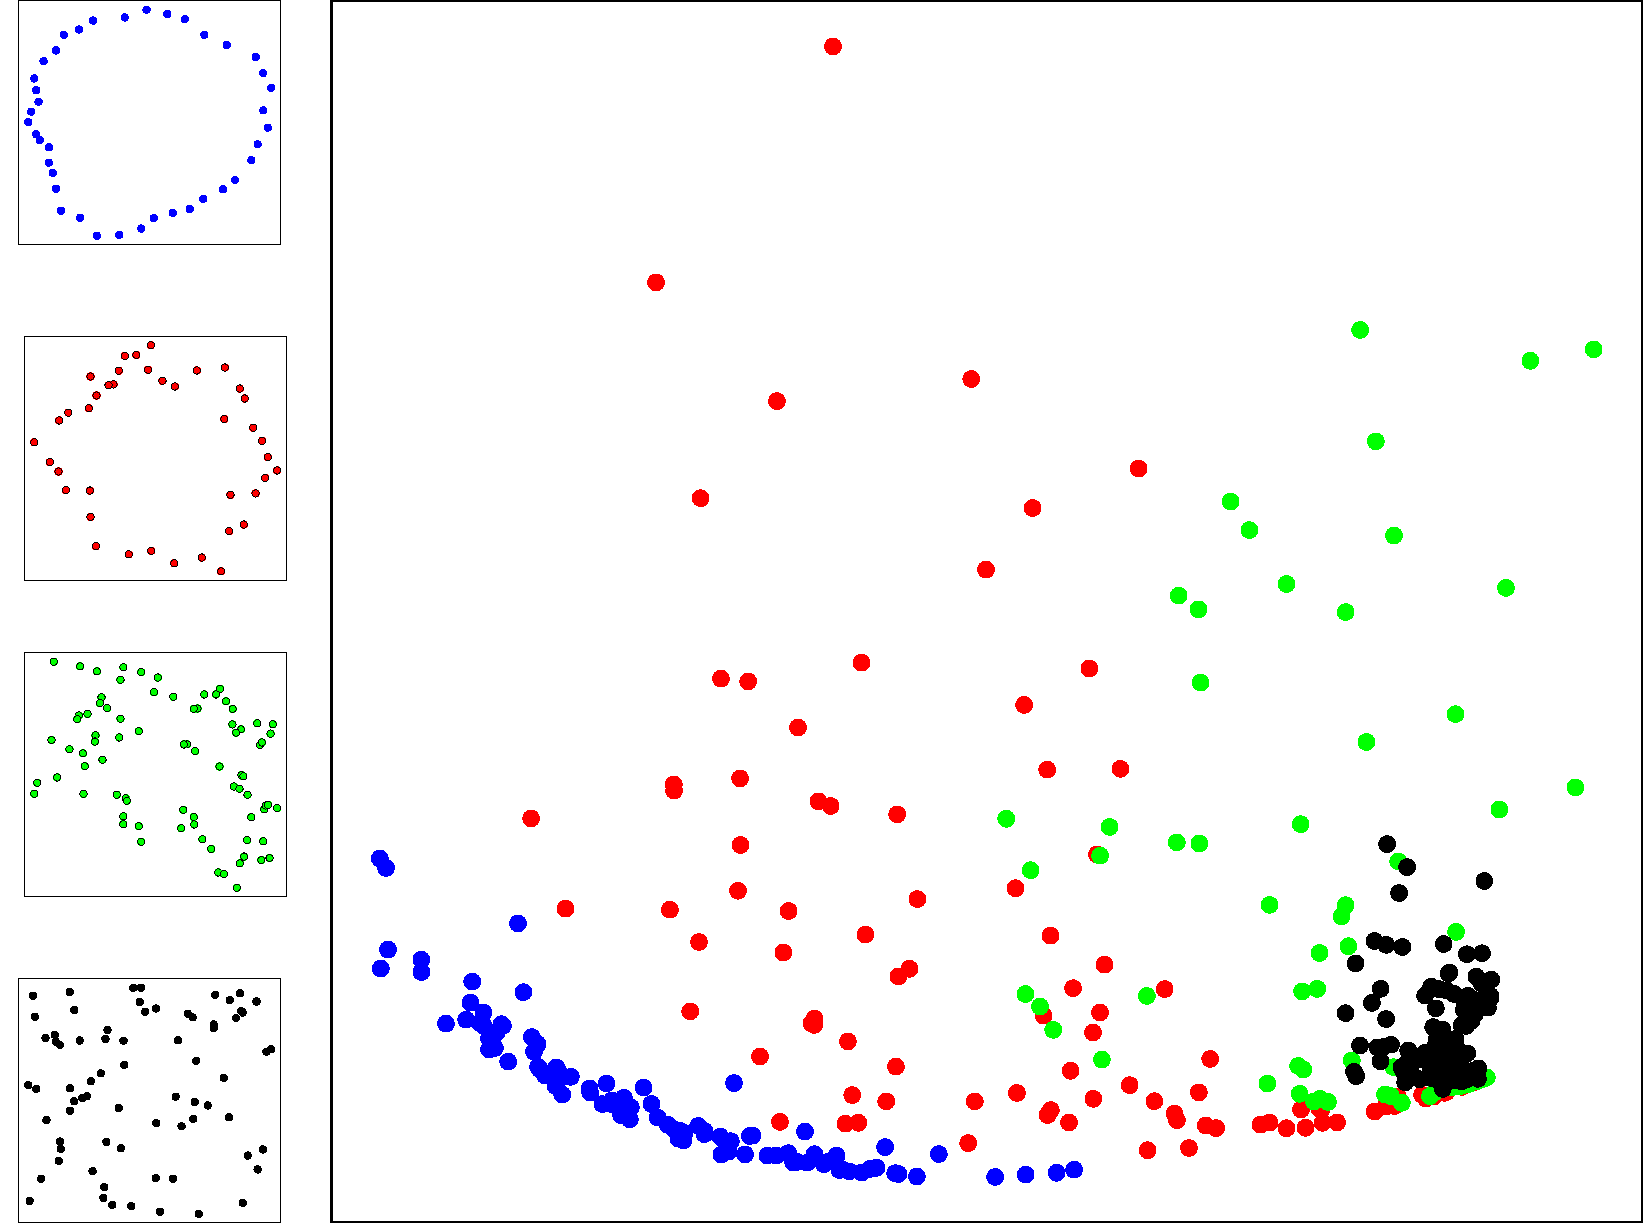
\includegraphics[height=2.5in]{gleason/sil-mds}}%
    \end{block}
\end{frame}

\begin{frame}
    \frametitle{Simulated Data}

    \begin{block}{}
        \begin{itemize}
            \item Training data: $2$k `glands', $500$ of each type
            \item Distance / DTM filtration
            \item Silhouette, $p=1$
            \item Test set: $400$, with $100$ of each type
            \item Remove labels from test set
            \item knn classification, with $k=3$
            \item $12\%$ classification error
        \end{itemize}
    \end{block}

\end{frame}

\againframe<1->{simulated}

\begin{frame}
    \frametitle{Real Data}
    \framesubtitle{Work with J.Q.\ Brown, C.\ Wenk, P.\ Lawson, A.\ Scholl. In
    submission.}

    \begin{block}{}
        \centering
        \only<1>{\includegraphics[height=2in]{gleason/tsne_fig_hist}}
    \end{block}
\end{frame}


